\chapter{Estudio Cinemático y Matemático} \label{chap:Cinematica}
\chapterimage{figuras/ImagenesPortada/PortadaCinematica.jpg}
\hrule
\vspace{3mm}

Este capítulo describe y desarrolla las relaciones matemáticas que definen los aspectos brazo robótico tal y como se ha descrito, principalmente la cinemática del robot.

\section{Cinemática del robot}

    La dificultad del problema cinemático del brazo tal y como se ha diseñado resulta bastante sencilla de obtener mediante métodos geométricos. Para ello se han descatado algunos ángulos y distancias en las figuras \ref{fig:Control:cinematica_1} y \ref{fig:Control:cinematica_1} que se calculan a continuación y que serán utilizadas para el cálculo de la cinemática directa e inversa.
    \\

    Debido a que el primer grado de libertad está desacoplado de los dos posteriores el estudio se puede separar, centrándose primeramente en el segundo y tercer grado de libertad.

    \begin{figure}[H]
        \centering
        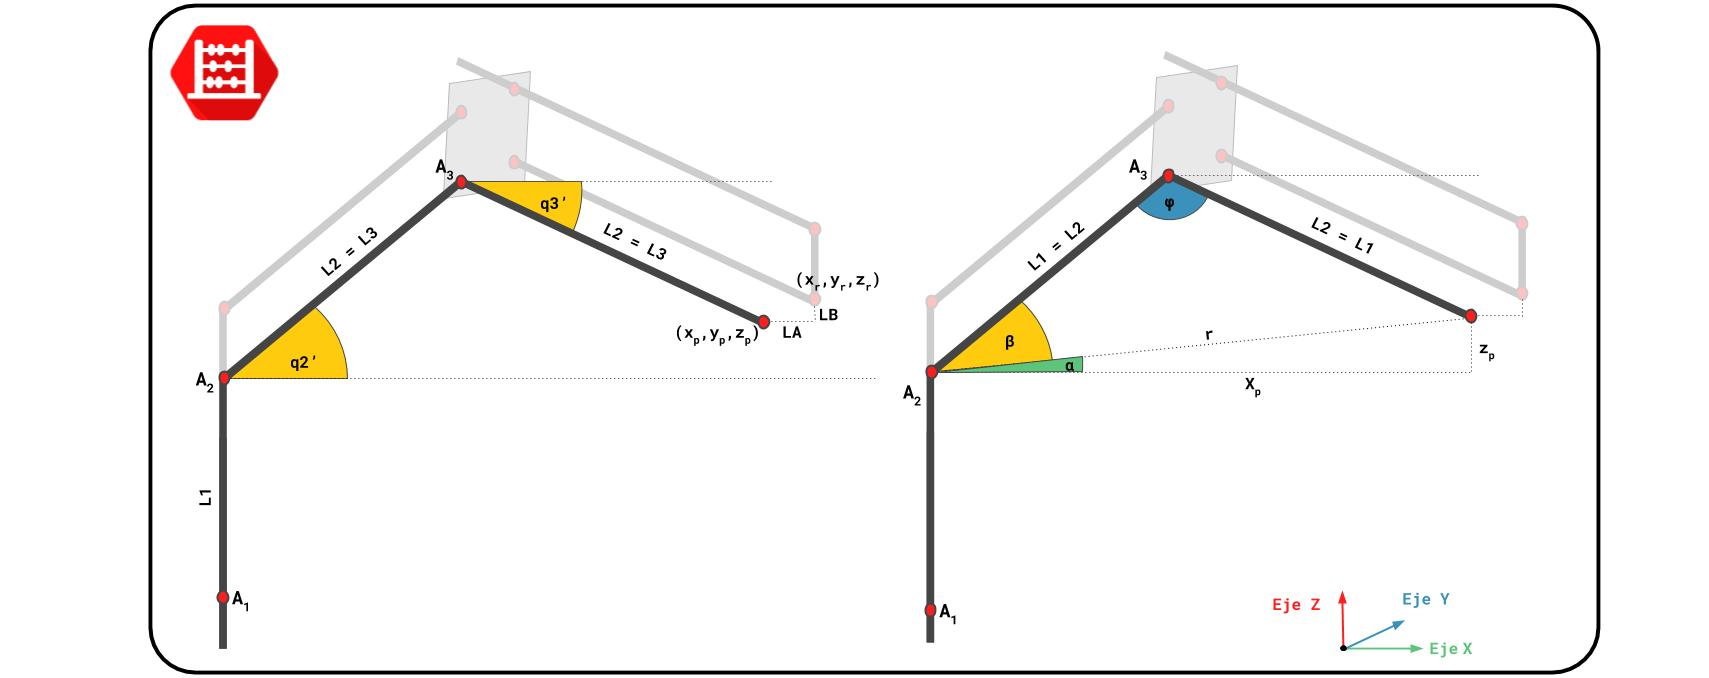
\includegraphics[width=1\textwidth]{figuras/Imagenes_cinematica/cinematica_1.jpg}
        \caption{Representación de los ángulos y distancias más representativas. GDL 2 y 3}
        \label{fig:Control:cinematica_1}
        \immagesource{Autor}
    \end{figure}



    \begin{equation}
        \alpha = \arctan\left(\frac{z_p}{x_p}\right)
    \end{equation}

    \begin{equation}
        \beta = \arccos\left(\frac{r^2+L2^2-L3^2}{2 \cdot L2 \cdot r}\right) = \arccos\left(\frac{r}{2 \cdot L2}\right)
    \end{equation}

    \begin{equation}
        \varphi = \arccos\left(\frac{L2^2+L3^2-r^2}{2 \cdot L2 \cdot L3}\right) = \arccos\left(\frac{r}{2L2}\right)
    \end{equation}

    \begin{equation}
        q_2' = \alpha + \beta
    \end{equation}

    \begin{equation}
        q_3' = \varPi - q_2' - \varphi
    \end{equation}

    \begin{equation}
        x_p = L2\cdot \cos(q_2') + L3\cdot \cos(q_3')
    \end{equation}

    \begin{equation}
        z_p = L2\cdot \sin(q_2') - L3\cdot \sin(q_3')
    \end{equation}

\subsection{Cinemática inversa}

    Teniendo las relaciones matemáticas genéricas obtenidas solo hay que adaptarlas a los ángulos que realmente se obtienen a través de los potenciómetros, estos ángulos son $q_2$ y $q_3$ en la figura \ref{fig:Control:cinematica_3}.

    \begin{figure}[H]
        \centering
        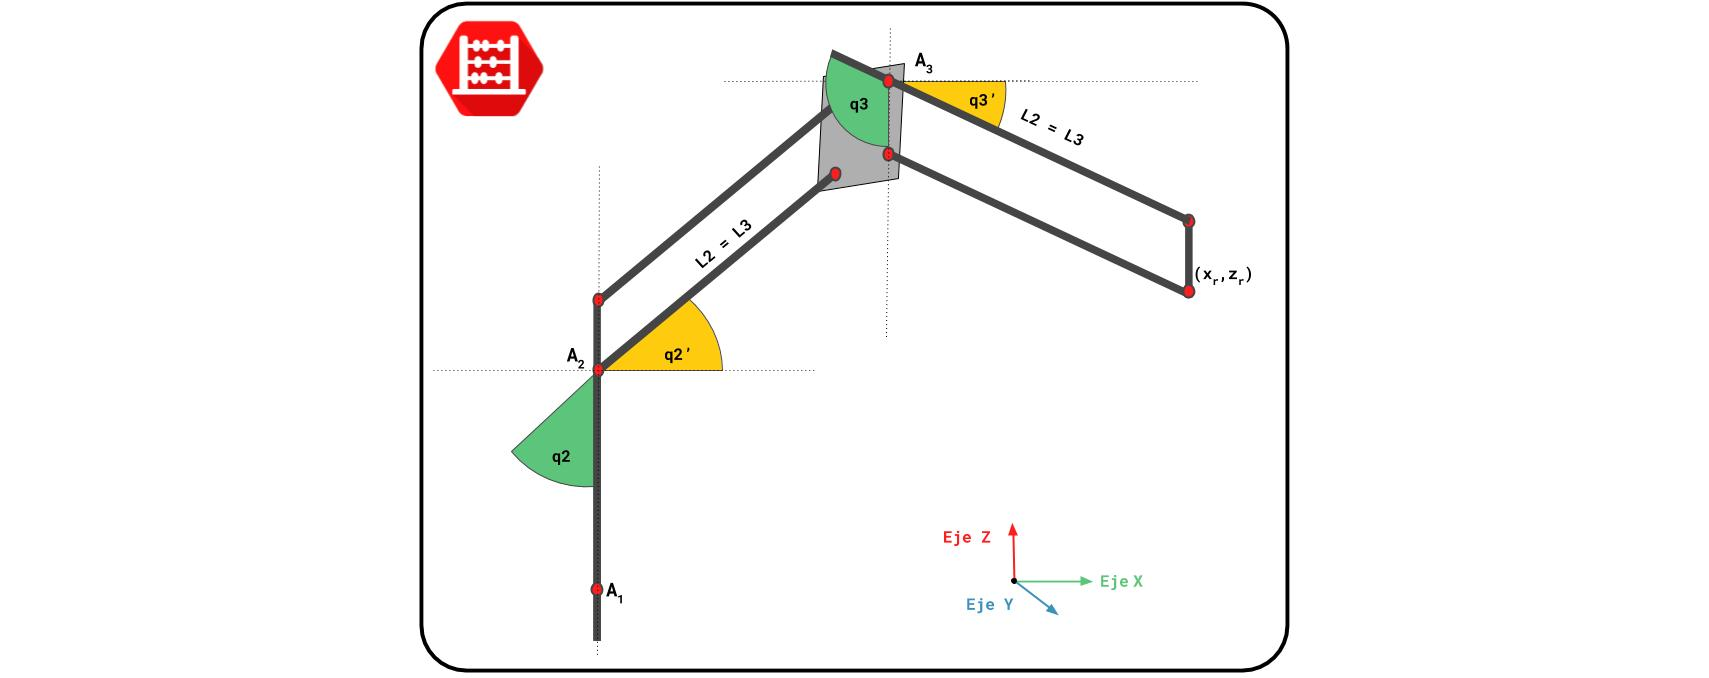
\includegraphics[width=1\textwidth]{figuras/Imagenes_cinematica/cinematica_3.jpg}
        \caption{Relación con los ángulos de interes}
        \label{fig:Control:cinematica_3}
        \immagesource{Autor}
    \end{figure}

    Además se debe tener en cuenta el primer grado de libertad, que no se ha representado anteriormente. En la figura \ref{fig:Control:cinematica_2} se puede ver con que criterio se ha tomado el ángulo en dicha articulación.

    \begin{figure}[H]
        \centering
        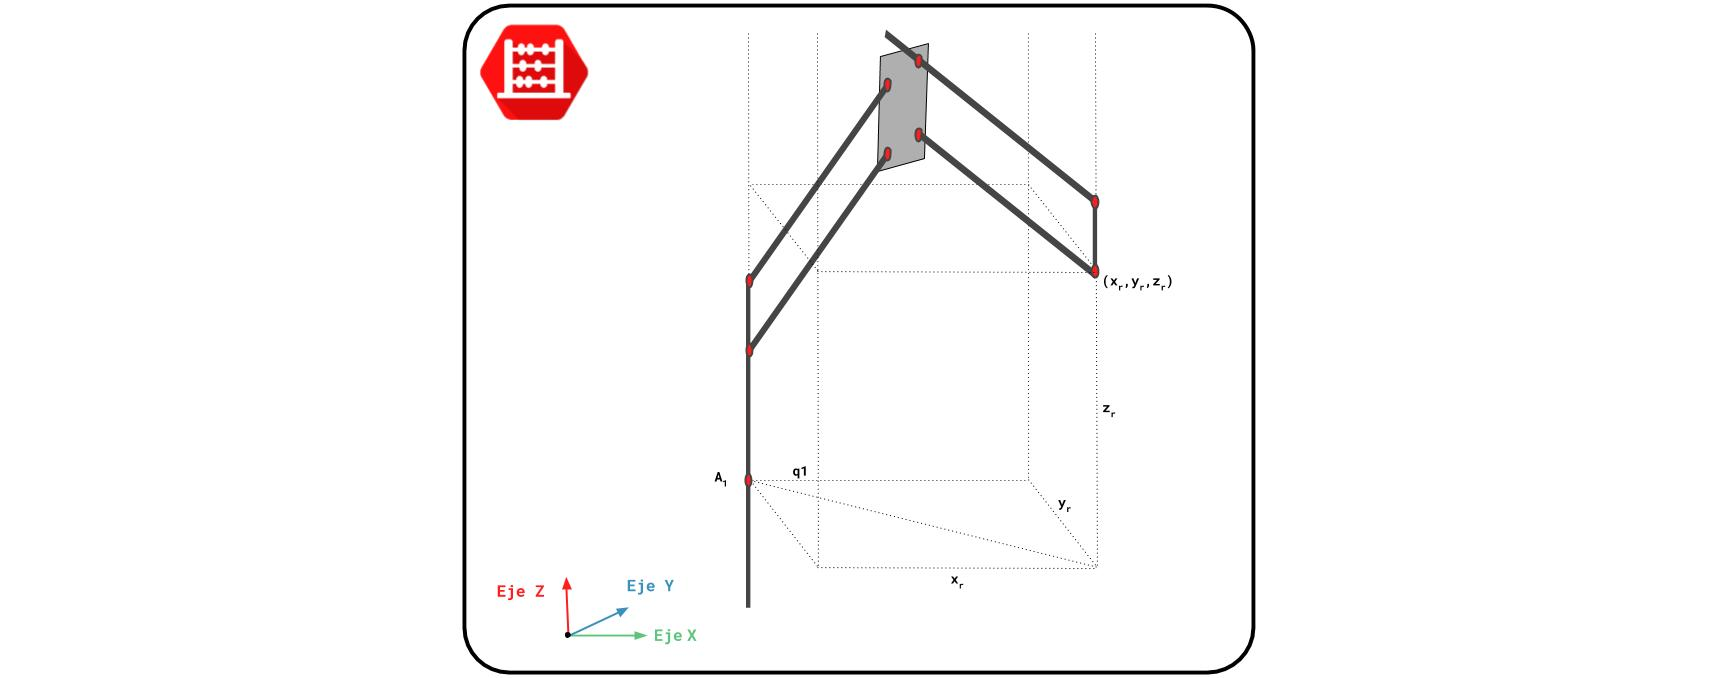
\includegraphics[width=1\textwidth]{figuras/Imagenes_cinematica/cinematica_2.jpg}
        \caption{Representación de los ángulos y distancias más representativas. Primer grado de libertad}
        \label{fig:Control:cinematica_2}
        \immagesource{Autor}
    \end{figure}

    De esta forma la cinemática inversa queda:

    \begin{equation}
        q_1 = \arctan\left(\frac{y_r}{x_r}\right)
    \end{equation}

    \begin{equation}
        q_2 = \frac{\varPi}{2} - q_2' = \frac{\varPi}{2} - \left(\arctan\left(\frac{z_p}{x_p}\right) + \arccos\left(\frac{r}{2 \cdot L2}\right)\right)
    \end{equation}

    \begin{equation}
        q_3 = q_3'- \frac{\varPi}{2} = \textnormal{\completar}
    \end{equation}


\subsection{Cinemática directa}

    Apoyándose en los cálculos realizados inicialmente la cinemática directa toma la siguiente forma:

    \begin{equation}
        x_r = x_p+LA = LA + L2 \cdot \left( \cos\left(\frac{\varPi}{2}-q_2\right) + \cos\left(q_3-\frac{\varPi}{2}\right) \right)
    \end{equation}

    \begin{equation}
        y_r = x_r \cdot \arctan{(q1)}
    \end{equation}

    \begin{equation}
        z_r = z_p+LB+L1 = LB + L1 + L2\cdot \left( \sin\left(\frac{\varPi}{2}-q_2\right) - \sin\left(q_3-\frac{\varPi}{2}\right) \right)
    \end{equation}

\subsection{Rango de movimiento en las articulaciones}


\section{Relación entre el par articular y del servo}
\completarCon{¿Como de imprescindible sería? Como dato está bien, pero realmente no es relevante para el control ni nada. TBD si hay tiempo}
\section{Relación entre la velocidad articular y del servo}
\completarCon{Igual que arriba}
	
\section{Realimentación articular}

	La relación entre las medidas angulares de los potenciómetros y de las articulaciones varían de una a otra. En ambos casos una vez transformado a ángulo articular habrá que aplicar el desfase para posicionar el cero angular en las posiciones descritas en la figura \ref{fig:Control:cinematica_3}. Hay que recordar de la sección \ref{sec:Electronica:Integracion} de qué manera se han integrado los potenciómetros en la estructura.
	
	   \begin{equation}
		   \textnormal{Segunda articulación:} \to	angulo_{articulacion} = angulo_{potenciometro} 
	   \end{equation}
	   
	   \begin{equation}
		   \textnormal{Tercera articulación:} \to	   angulo_{articulacion} = angulo_{potenciometro} \cdot 0.679
	   \end{equation}